\documentclass{article}
\usepackage[utf8]{inputenc}
\usepackage[spanish]{babel}
\usepackage{graphicx}
\usepackage{natbib}  % Usando paquete para citas 
\usepackage{amsmath}
\usepackage{amssymb}

\bibliographystyle{acl_natbib}  % Cargando estilo de bibliografia
\graphicspath{{./img/}}
\title{Propuesta de Tesis}
\author{Diego Alberto Barriga Martínez}
\date{Julio 2019}

\begin{document}
\maketitle
\tableofcontents
\newpage
\section{Título de tesis}
\textbf{Etiquetador automático de la morfología del otomí usando predicción estructurada}

\section{Objetivo de la propuesta}
Diseñar e implementar un etiquetador morfológico para el otomí basado en
técnicas de Procesamiento del Lenguaje Natural (Natural Language Processing,
NLP) con Aprendizaje de Máquina (Machine Learning, ML). En particular, se hará
énfasis en métodos de aprendizaje estructurado débilmente supervisados.
Específicamente, se aplicará Conditional Random Fields (CRF) para etiquetado
morfológico (glosado) del otomí, una lengua de bajos recursos.

\section{Definición del problema}
El NLP es un área de la computación que permite reconocer, procesar e
interpretar el lenguaje humano dentro de un sistema computacional. El objetivo
de esta área es hacer que las computadoras realicen tareas que involucran el
lenguaje humano. Algunas tareas generales consisten en permitir la comunicación
humano-máquina, o simplemente hacer un exitoso procesamiento de texto o voz
humanos. (Jurafsky \& Martin, 2014). Ejemplos de aplicación actuales son los
traductores automáticos, asistentes personales que reconocen voz, motores de
búsquedas en Internet, análisis de sentimientos en textos,  síntesis de voz,
etiquetado de textos y muchas más aplicaciones.

Una de las tareas más populares de NLP es el etiquetado automático de textos.
Este etiquetado puede realizarse a diferentes niveles lingüísticos, por
ejemplo, morfosintáctico (Part-Of-Speech tagging), sintáctico (parsing),
morfológico, etc.  El nivel morfológico tiene que ver con la estructura interna
de las palabras (Haspelmath y Sims, 2013); en particular, existe un tipo de
etiquetado, de gran importancia para el análisis lingüístico, llamado glosado
que asigna etiquetas a las unidades que conforman a una palabra. 

Para lograr lo anterior, los enfoques actuales aplican técnicas de ML. El ML es
un subcampo de la Inteligencia Artificial (IA), que constituye un enfoque de
resolución de problemas caracterizado por estimar una solución a partir de la
experiencia (Mitchell, 1997).  La experiencia se refiere a datos etiquetados
(ejemplos) que permiten inferir un modelo estadístico de aprendizaje. Entre los
métodos de ML ampliamente utilizados se pueden mencionar las Support Vector
Machines (SVMs), árboles de decisión, o bien los modelos gráficos, como las
redes neuronales o los métodos generativos, solo por mencionar algunos. Para
las tareas de etiquetado en NLP generalmente se utilizan modelos gráficos
supervisados, por ejemplo, modelos ocultos de Markov (Hidden Markov Models,
HMM).

No obstante, el lenguaje natural es complejo y dinámico, ya que tiene fenómenos
que hacen que las tareas de reconocimiento, generación y procesamiento se
vuelvan difíciles para las computadoras. Adicionalmente, existen escenarios
donde estos métodos no son efectivos como es el caso de las lenguas de bajos
recursos, que son lenguas que tienen pocos recursos digitales con los que
trabajar. Por ejemplo, si se tienen pocos datos iniciales para el entrenamiento
del modelo de aprendizaje las predicciones serán poco precisas o equivocadas.
Los bajos recursos son un escenario común en México donde, a pesar de que
existe una rica diversidad lingüística, gran parte de las lenguas originarias
no poseen contenido web ni publicaciones digitales y por tanto carecen también
de tecnologías del lenguaje.  El escenario mencionado anteriormente supone un
reto para los métodos de aprendizaje convencionales, que requieren de grandes
cantidades de datos de entrenamiento para funcionar correctamente. Por lo
tanto, es un importante reto de investigación desarrollar aproximaciones que
funcionen con lenguas de escasos recursos. En particular, nos enfocaremos en el
glosado automático del  otomí, una lengua con gran riqueza morfológica y con
escasez de recursos digitales.

El glosado puede ser un primer paso para el desarrollo de más tecnologías del
lenguaje; no solo para el otomí, que presenta un grado de extinción acelerada
(CDI), sino para las 68 agrupaciones lingüísticas que se hablan en México.

\section{Metodología}
Se pretende utilizar un método gráfico, Conditional Random Fields (CRFs), que
permita predecir secuencias de etiquetas (aprendizaje estructurado) para
describir las unidades morfológicas dentro de una palabra del otomí. El
aprendizaje estructurado predice elementos secuenciales basándose en las
secuencias previamente vistas en el entrenamiento. A grandes rasgos, este tipo
de aprendizaje consiste en hacer predicciones de secuencias estructuradas
maximizando una función de error. Tal función de compatibilidad se da entre una
entrada X y un conjunto de posibles etiquetas Y generadas por el modelo de ML.
En este trabajo, se pretende generar de forma automática una secuencia de
etiquetas, conocidas como glosa para el otomí. 

Utilizaremos los CRFs para predecir secuencias de glosas dada la observación de
secuencias de entrada. Se considera exitosa la predicción si se logra maximizar
la correcta clasificación de las secuencias de salida.  En principio, las
variables dependen unas de otras y una forma de representar dicha dependencias
son con modelos basados en grafos. 

Para satisfacer las secuencias de entrada se deben tener disponibles datos de
entrenamiento. En este trabajo se necesita un corpus del otomí que, además,
cumpla la característica de estar glosado. Glosar es una tarea difícil y
requiere del trabajo exhaustivo de un especialista (lingüistas) y hablantes
nativos. Se tomará el corpus Tsunkua (Elotl, 2019) etiquetado por el lingüista
Víctor Germán Mijangos de la Cruz y que está basado en el trabajo El otomí de
Toluca (Lastra, 1992). 

Una vez obtenido los datos se realizará el preprocesamiento y análisis del
corpus.  Es importante mencionar que el corpus a utilizar esta apegado a las
normas ortográficas para el otomí establecidas por el Instituto Nacional de
Lenguas Indígenas (INALI, 2014). Una vez terminado el preprocesamiento se
realizará la optimización de hiperparametros de la arquitectura atendiendo las
necesidades del otomí. Por último, se llevarán a cabo una serie de etapas de
prueba, evaluación y análisis de resultados. 

\section{Inventario de materias/temas de la carrera que se utilizarán para el desarrollo de seminario/tesis}

\begin{itemize}
    \item Álgebra Líneal
    \item Probabilidad y Estadística
    \item Cálculo Vectorial
    \item Estructuras Discretas
    \item Leguajes Formales y Autómatas
    \item Procesamiento de Lenguaje Natural
    \item Aprendizaje de Máquina
    \item Temas Selectos de Tecnología del Lenguaje
    \item Análisis y Procesamiento Inteligente de Textos
\end{itemize}

\section{Índice desglozado}
\begin{itemize}
    \item Introducción
    \begin{itemize}
        \item Problemática
        \item Objetivo
        \item Hipótesis
    \end{itemize}
    \item Avances en etiquetadores automáticos
    \begin{itemize}
        \item Marco teórico
        \item Estado del arte
    \end{itemize}
    \item Etiquetador morfológico para el otomí (Metodología)
    \begin{itemize}
        \item CRFs
        \item Definición de la arquitectura
        \item Features
    \end{itemize}
    \item Resultados y análisis de resultados
    \item Conclusiones
    \begin{itemize}
        \item Trabajo futuro
    \end{itemize}
    \item Referencias
\end{itemize}

\section{Resultados esperados} \label{sec:resultados}
Se espera obtener un modelo que produzca glosa para el otomí, generada
automáticamente, con base en el entrenamiento con pocos ejemplos previamente
etiquetados. Al obtener una buena exactitud en la predicción automática de
glosa se apoyaría a los anotadores humanos a reducir trabajo repetitivo y
exhaustivo. Además, se espera obtener avances de una metodología adaptable a un
mayor número de lenguas mexicanas. Sería deseable que esta metodología
experimental pueda ser replicable en otras lenguas habladas en México. Se puede
ver en los resultados del cuadro \ref{tab:tabla1}. Se vio en el capitulo
\ref{sec:resultados} y con base en el cronograma de la figura \ref{fig:cronograma}

\begin{table}[]
    \centering
    \begin{tabular}{|c|c|c|}
        \hline \bf valor & \bf score & \bf label \\
        \hline 0.43 & 0.99 & oto \\
        \hline 0.23 & 0.65 & esp \\
    \end{tabular}
    \caption{Resultados}
    \label{tab:tabla1}
\end{table}{}


$ a = b  \mathbb{RN} $

\section{Cronograma de actividades}
\begin{figure}
    \centering
    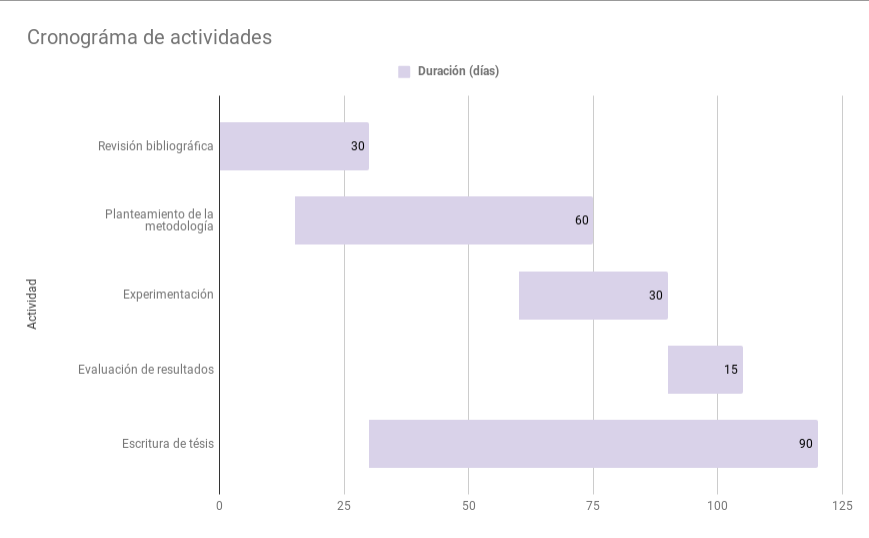
\includegraphics[width=\textwidth]{crono.png}
    \caption{Cronograma}
    \label{fig:cronograma}
\end{figure}{}

%\citep{walker1974new}  % Cita indirecta
%\citet{zou2013bilingual} % cita directa 

\bibliography{xim-ref}  % Archivo donde estan las referencias

\end{document}
  
